\section{Review: Continuity, Distance, and Linear Algebra Review}
\textit{Lecture 2 and 3 (Sept 13 and 15) + Tutorial 1}
\begin{itemize}
    \item The properties in the previous section will be important when giving a formal definition of continuity.
          \begin{definition}
              If $x,y\in \mathbb{R}^n$, then:
              \begin{equation}
                  d(x,y) = \text{``Distance between $x$ and $y$''} = |x-y|
              \end{equation}
          \end{definition}
          \begin{theorem}
              \begin{enumerate}
                  \item $d$ is \textbf{symmetric}, i.e. $d(x,y)=d(y,x)$.
                  \item $d$ is \textbf{positive definite}, i.e. $d(x,y) \ge 0$ and $d(x,y)=0 \iff x=y$.
                  \item Triangle Inequality: $d(x,z) \le d(x,y) + d(y,z).$
              \end{enumerate}
          \end{theorem}
          \begin{proof}
              We prove each separately:
              \begin{enumerate}
                  \item $d(x,y) = |x-y| = |-(y-x)| = |-1| \cdot |y-x| = |y-x| = d(y,x)$
                  \item $d(x,y) = 0 \iff |x-y| = 0 \iff x-y = 0 \iff x=y$
                  \item We need to check that
                        \begin{align}
                            d(x,z) & \stackrel{?}{\le} d(x,y) + d(y,z) \\
                            |x-z|  & \stackrel{?}{\le} |x-y| + |y-z|   \\
                            |x-z|  & \stackrel{?}{\le} |x-z|
                        \end{align}
                        where the third line comes from the previous triangle inequality. The last statement is true, and the steps are reversible, so we are done.
              \end{enumerate}
          \end{proof}
    \item This theorem is significant as these are the only properties that we need to know about distances to formally define continuity.

          \textit{Note:} In a future section, we will use these properties to \textit{define} a distance function (formally a metric), which is anything that satisfies these properties. This will allow us to generalize continuity to more abstract spaces.
    \item A note on notation. Our definition of a norm is known as the $L^2$ or \textit{Euclidean norm,} i.e.
          \begin{equation}
              |x|_{L^2} = \sqrt{\sum x_i^2}
          \end{equation}
          The $L^1$ norm can be defined as
          \begin{equation}
              |x|_{L^1} = \sum |x_i|
          \end{equation}
          and the infinity norm:
          \begin{equation}
              |x|_\infty = \text{sup}|x_i|.
          \end{equation}
          which is the maximum coordinate. Note that for a finite space, we can use $\text{max}$, but the use of supreme allows us to generalize to infinite spaces.
          \begin{idea}
              The $p$-norm can be defined as
              \begin{equation}
                  |x|_{L^p} = \left(\sum x_i^p\right)^{1/p}
              \end{equation}
              And it turns out that
              \begin{equation}
                  |x|_{\infty} = \lim_{p\to\infty} |x|_{L^p}.
              \end{equation}
              There is a nice geometric idea behind why this is the case. Consider $\mathbb{R}^2$. Then we can plot vectors with a norm of $1$ in $L^1,L^2,L^3$ where the coordinate axes are $x_1$ and $x_2$.
              \begin{center}
                  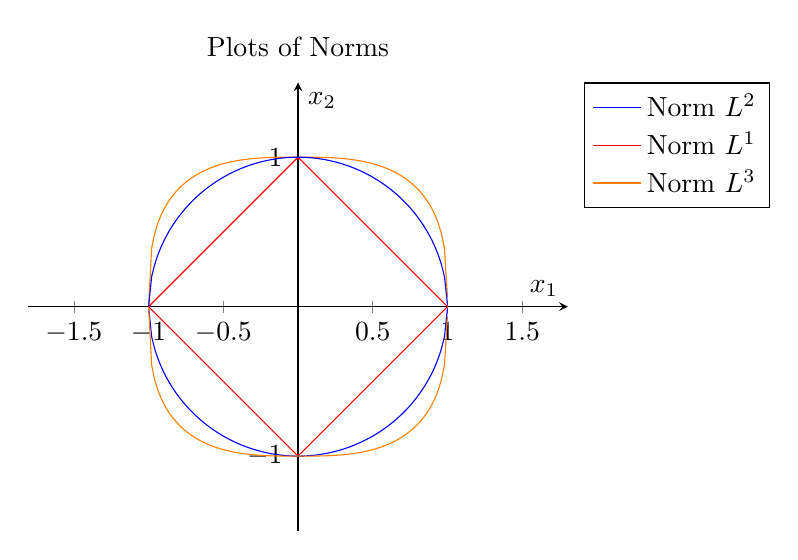
\begin{tikzpicture}
                      \begin{axis}[
                              legend pos=outer north east,
                              title=Plots of Norms,
                              axis lines = middle,
                              xlabel = $x_1$,
                              ylabel = $x_2$,
                              variable = t,
                              trig format plots = rad,
                              axis equal,
                              xmin= -1.5,
                              xmax = 1.5,
                              ymin = -1.5,
                              ymax = 1.5,
                          ]
                          \addplot [
                              domain=-1:1,
                              samples=100,
                              color=blue,
                          ]
                          {-sqrt(1-x^2)};
                          \addlegendentry{Norm $L^2$}
                          \addplot [
                              domain=-1:1,
                              samples=100,
                              color=red,
                          ]
                          {abs(x)-1};
                          \addlegendentry{Norm $L^1$}
                          \addplot [
                              domain=-1:1,
                              samples=100,
                              color=orange,
                          ]
                          {(1-abs(x)^3)^(1/3)};
                          \addlegendentry{Norm $L^3$}
                          \addplot [
                              domain=-1:1,
                              samples=100,
                              color=orange,
                          ]
                          {-(1-abs(x)^3)^(1/3)};
                          \addplot [
                              domain=-1:1,
                              samples=100,
                              color=red,
                          ]
                          {1-abs(x)};
                          \addplot [
                              domain=-1:1,
                              samples=100,
                              color=blue,
                          ]
                          {sqrt(1-x^2)};
                      \end{axis}
                  \end{tikzpicture}
              \end{center}
              We can see that as the dimension of the norm increases, the plot becomes closer and closer to a square, which can be represented by $\max\{x_1,x_2\}$.
          \end{idea}
          \begin{example}
              Suppose we have $\lVert \cdot \rVert_a$ on $\mathbb{R}^n$ and a norm $\lVert \cdot \rVert_b$ on $\mathbb{R}^n$. Suppose $\exists c > 0$ such that $\lVert x\rVert_b \le c \lVert x\rVert_a.$ Then if $f:\mathbb{R}^n \rightarrow \mathbb{R}$ is continuous with respect to the $b$-norm, then it is also continuous with respect to the $a$-norm.
              \begin{proof}
                  We know that for any $\epsilon > 0,$ we have $\lVert x-y\rVert_b < \delta_b \implies |f(x)-f(y)| < \epsilon.$ Let us pick $\delta = \frac{\delta_b}{c}$. Then we have:
                  \begin{align}
                      \lVert x-y\rVert_a < \frac{\delta_b}{c} &\implies c\lVert x-y\rVert_a < \delta_b \\ 
                      &\implies \lVert x-y\rVert_b \le c\lVert x-y\rVert_a < \delta_b \\ 
                      &\implies |f(x)-f(y)| < \epsilon 
                  \end{align}
              \end{proof}
          \end{example}
    \item Similarly, distances for $L^1$ and the infinity norms can be defined as $d_1(x,y)=|x-y|_1$ and $d_\infty(x,y)=|x-y|_\infty$.

          \textbf{Exercise:} Show that $d_1$ and $d_\infty$ also satisfy the properties of a distance.

    \item There is a bijection from the linear map $\mathbb{R}^n \to \mathbb{R}^m$ and a $m\times n$ matrix:
          \begin{equation}
              \left\{T:\mathbb{R}^n \to \mathbb{R}^m\right\} \longleftrightarrow M_{m\times n}(\mathbb{R})
          \end{equation}
          which is also a homomorphism. We can associate a matrix with any linear transformation, and any linear transformation is associated with a matrix. Here, the standard basis is used.
    \item Specifically, we have the map:
          \begin{equation}
              A \in M_{m\times n} \mapsto     L_A(x)= Ax
          \end{equation}
          where $x\in \mathbb{R}^n$, and
          \begin{equation}
              T \mapsto M_T = \begin{pmatrix}
                  Te_1 & Te_2 & \cdots & Te_n
              \end{pmatrix}
          \end{equation}
    \item We also need to show that this map is bijective, i.e both
          \begin{equation}
              L_{M_T}=T,\quad M_{L_A}=A
          \end{equation}
          are both satisfied.
    \item Furthermore, we can also show that this map is a homomorphism. Note that the set of linear transformations is itself a vector space. Both $A\mapsto L_A$ and $T\mapsto M_T$ is linear, so
          \begin{align}
              L_{aA+bB} & = aL_A + bL_b \\
              M_{aT+bS} & = aM_T+bM_s.
          \end{align}
    \item Furthermore, suppose we have two maps $T:\mathbb{R}^n \rightarrow \mathbb{R}^m$ and $S:\mathbb{R}^m \rightarrow \mathbb{R}^p$. To go from $\mathbb{R}^n$ to $\mathbb{R}^p$, we can take the composition
          \begin{equation}
              S \circ T
          \end{equation}
          or
          \begin{equation}
              S \sslash T
          \end{equation}
          The bijection is a homomorphism, so we have
          \begin{equation}
              M_S M_T = M_{S \circ T}
          \end{equation}
\end{itemize}